\section{Análise sintática preditiva não-recursiva}

\begin{frame}[fragile]{Analisador preditivo não-recursivo}

    \begin{itemize}
        \item É possível construir um analisador sintático preditivo não-recursivo, no qual as chamadas recursivas são eliminadas por meio do uso de uma
            pilha explícita
       %\pause

        \item Seja recursivo ou não, o principal problema a ser resolvido por um analisador sintático é o de identificar a produção que deve ser aplicada a
            um não-terminal
       %\pause

        \item Um analisador sintático não-recursivo busca em uma tabela sintática pela produção a ser aplicada
       %\pause

        \item Tal tabela pode ser construída diretamente a partir de certas gramáticas
    \end{itemize}

\end{frame}

\begin{frame}[fragile]{Modelo de um analisador sintático preditivo não-recursivo}

    \begin{figure}
        \centering
        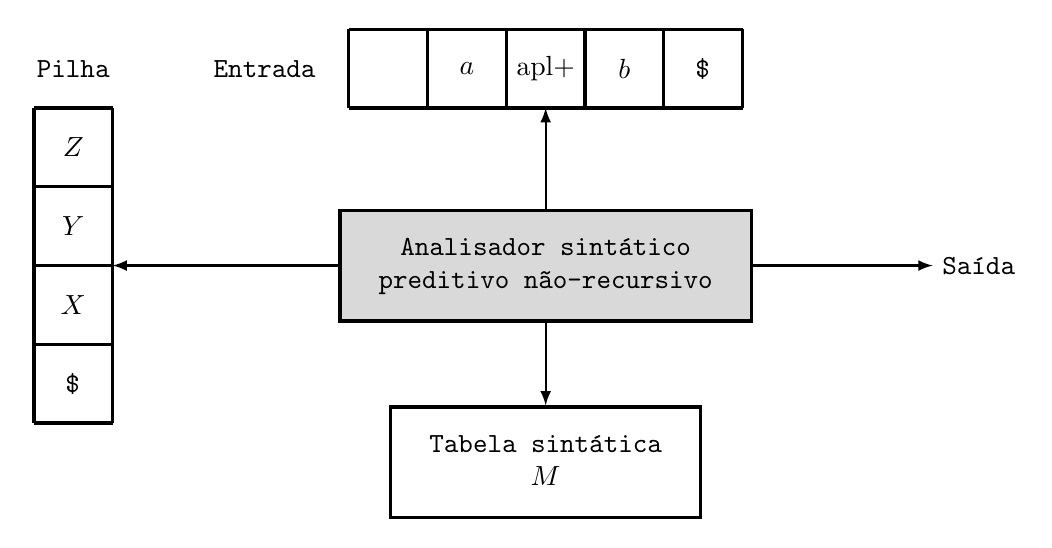
\begin{tikzpicture} 
            \node[draw,very thick,fill=gray!30,inner sep=8pt] (A) at (6.5, 3) { \texttt{\begin{tabular}{c} Analisador sintático\\ preditivo não-recursivo\end{tabular}} };
            \node[draw,very thick,inner sep=8pt] (B) at (6.5, 0.5) { \texttt{\begin{tabular}{c} Tabela sintática\\ $M$\end{tabular}} };
            \draw[very thick] (4, 5) grid (9, 6);
            \draw[very thick] (0, 1) grid (1, 5);

            \node (C) at (12, 3) { \texttt{Saída} };

            \node[anchor=east] at (3.7, 5.5) { \texttt{Entrada} };
            \node at (0.5, 5.5) { \texttt{Pilha} };

            \node at (0.5, 1.5) { \texttt{\$} };
            \node at (0.5, 2.5) { $X$ };
            \node at (0.5, 3.5) { $Y$ };
            \node at (0.5, 4.5) { $Z$ };

            \node at (5.5, 5.5) { $a$ };
            \node at (6.5, 5.5) { \code{apl}{+} };
            \node at (7.5, 5.5) { $b$ };
            \node at (8.5, 5.5) { \texttt{\$} };

            \draw[thick,-latex] (A) to (B);
            \draw[thick,-latex] (A) to (6.5, 5);
            \draw[thick,-latex] (A) to (1, 3);
            \draw[thick,-latex] (A) to (C);
        \end{tikzpicture} 
    \end{figure}

\end{frame}

\begin{frame}[fragile]{Estrutura de um analisador sintático preditivo não-recursivo}

    \begin{itemize}
        \item Um analisador sintático preditivo não-recursivo é composto por um \textit{buffer} de entrada, uma pilha, uma tabela sintática e um fluxo de saída
       %\pause

        \item O \textit{buffer} de entrada contém a cadeia a ser analisada, seguida de um sentinela que indique o fim da cadeia (assuma que o sentinela é o
            caractere \texttt{\$})
       %\pause

        \item A pilha contém símbolos gramaticais, onde o sentinela indica o fundo da pilha
       %\pause

        \item Inicialmente a pilha deve contém o símbolo de partida da gramática logo acima do sentinela
       %\pause
    
        \item A tabela sintática é uma matriz $M[A, a]$ cuja primeira dimensão contém não-terminais $A$ e a segunda contém terminais $a$ ou o sentinela
            \texttt{\$}
    \end{itemize}

\end{frame}

\begin{frame}[fragile]{Algoritmo para o analisar sintático preditivo não-recursivo}

    \begin{algorithmic}[1]
        \Require{Uma cadeia $w$ e uma tabela sintática $M$ para uma gramática $G$}
        \Ensure{Se $w\in L(G)$, uma derivação mais à esquerda de $w$, caso contrário sinaliza um erro}

        \vspace{0.1in}

        \State{$a\gets$ primeiro símbolo de $w$}
        \Repeat
            \State{$X\gets$ topo da pilha}
            \If{$X$ é um terminal}
                \If{$X = a$}
                    \State{remova $X$ da pilha}
                    \State{$a\gets$ próximo símbolo de $w$}
                \Else
                    \State{sinalize um erro}
                \EndIf
            \algstore{bkbreak}
    \end{algorithmic}

\end{frame}

\begin{frame}[fragile]{Algoritmo para o analisar sintático preditivo não-recursivo}

    \begin{algorithmic}[10]
        \algrestore{bkbreak}
            \ElsIf{$X$ é um não-terminal}
                \If{$M[X, a] = X \to Y_1Y_2\ldots Y_k$}
                    \State{remova $X$ da pilha}
                    \State{empilhe $Y_k, Y_{k - 1}, \ldots, Y_1$, com $Y_1$ no topo da pilha}
                    \State{escreva a produção $X \to Y_1Y_2\ldots Y_k$ na saída}
                \Else
                    \State{sinalize um erro}
                \EndIf
            \EndIf
        \Until{$X = $ \texttt{\$}}
    \end{algorithmic}

\end{frame}

\begin{frame}[fragile]{Tabela sintática para a gramática de expressões aritméticas}

    \begin{table}
        \centering
        \begin{tabular}{c|c|c|c|c|c|c}
        \toprule
        \multirow{2}{*}{\texttt{\begin{tabular}{c}Não-\\ terminal\end{tabular}}} & \multicolumn{6}{c}{\texttt{Símbolo da entrada}} \\
        \cmidrule{2-7}
        & \textbf{id} & \code{apl}{+} & \code{apl}{×} & $($ & $)$ & \texttt{\$} \\
        \midrule
        $E$ & $E\to TE'$ & & & $E\to TE'$ & \\
        \rowcolor[gray]{0.9}
        $E'$ & & $E'\to \code{apl}{+}TE'$ & & & $E'\to \code{apl}{∊}$ & $E'\to \code{apl}{∊}$ \\
        $T$ & $T\to FT'$ & & & $T\to FT'$ & \\
        \rowcolor[gray]{0.9}
        $T'$ & & $T'\to \code{apl}{∊}$ & $T'\to \code{apl}{×}FT'$ & & $T'\to \code{apl}{∊}$ & $T'\to \code{apl}{∊}$ \\
        $F$ & $F\to \textbf{id}$ & & & $F\to (E)$ & & \\
        \bottomrule
        \end{tabular}
    \end{table}

\end{frame}

\begin{frame}[fragile]{Comportamento do analisador preditivo não-recursivo para a cadeia ``$\textbf{id}\code{apl}{+}\textbf{id}\code{apl}{×}\textbf{id}$''}

    \begin{tikzpicture}
        \node[opacity=0] at (12, 0) { . };
        \node[opacity=0] at (12, 7) { . };

        \node at (2.5, 0.5) { \texttt{Pilha} };

        \draw[very thick] (1.5, 1) to (3.5, 1);

        \draw[thick] (2, 1) rectangle (3, 2);
        \node at (2.5, 1.5) { \texttt{\$} };

        \draw[thick] (2, 2) rectangle (3, 3);
        \node at (2.5, 2.5) { $E$ };

        \node[anchor=west] at (5, 5) { \texttt{Entrada} };

        \node[anchor=west] at (6, 4) { \textbf{id} \code{apl}{+} \textbf{id} \code{apl}{×} \textbf{id} \texttt{\$} };

        \node[anchor=west] at (10, 5) { \texttt{Saída} };

%        \node[anchor=west] at (11, 4) { $E'\to \code{apl}{+}TE'$ };
    \end{tikzpicture}

\end{frame}

\begin{frame}[fragile]{Comportamento do analisador preditivo não-recursivo para a cadeia ``$\textbf{id}\code{apl}{+}\textbf{id}\code{apl}{×}\textbf{id}$''}

    \begin{tikzpicture}
        \node[opacity=0] at (12, 0) { . };
        \node[opacity=0] at (12, 7) { . };

        \node at (2.5, 0.5) { \texttt{Pilha} };

        \draw[very thick] (1.5, 1) to (3.5, 1);

        \draw[thick] (2, 1) rectangle (3, 2);
        \node at (2.5, 1.5) { \texttt{\$} };

        \draw[thick] (2, 2) rectangle (3, 3);
        \node at (2.5, 2.5) { $E$ };

        \node[anchor=west] at (5, 5) { \texttt{Entrada} };

        \node[anchor=west] at (6, 4) { \textbf{id} \code{apl}{+} \textbf{id} \code{apl}{×} \textbf{id} \texttt{\$} };
        \draw[-latex,thick] (6.3, 3.2) to (6.3, 3.8);

        \node[anchor=west] at (10, 5) { \texttt{Saída} };

%        \node[anchor=west] at (11, 4) { $E'\to \code{apl}{+}TE'$ };
    \end{tikzpicture}

\end{frame}

\begin{frame}[fragile]{Comportamento do analisador preditivo não-recursivo para a cadeia ``$\textbf{id}\code{apl}{+}\textbf{id}\code{apl}{×}\textbf{id}$''}

    \begin{tikzpicture}
        \node[opacity=0] at (12, 0) { . };
        \node[opacity=0] at (12, 7) { . };

        \node at (2.5, 0.5) { \texttt{Pilha} };

        \draw[very thick] (1.5, 1) to (3.5, 1);

        \draw[thick] (2, 1) rectangle (3, 2);
        \node at (2.5, 1.5) { \texttt{\$} };

        \draw[thick] (2, 2) rectangle (3, 3);
        \node at (2.5, 2.5) { $E'$ };

        \draw[thick] (2, 3) rectangle (3, 4);
        \node at (2.5, 3.5) { $T$ };

        \node[anchor=west] at (5, 5) { \texttt{Entrada} };

        \node[anchor=west] at (6, 4) { \textbf{id} \code{apl}{+} \textbf{id} \code{apl}{×} \textbf{id} \texttt{\$} };
        \draw[-latex,thick] (6.3, 3.2) to (6.3, 3.8);

        \node[anchor=west] at (10, 5) { \texttt{Saída} };

        \node[anchor=west] at (11, 4) { $E\to TE'$ };
%        \node[anchor=west] at (11, 4) { $E'\to \code{apl}{+}TE'$ };
    \end{tikzpicture}

\end{frame}

\begin{frame}[fragile]{Comportamento do analisador preditivo não-recursivo para a cadeia ``$\textbf{id}\code{apl}{+}\textbf{id}\code{apl}{×}\textbf{id}$''}

    \begin{tikzpicture}
        \node[opacity=0] at (12, 0) { . };
        \node[opacity=0] at (12, 7) { . };

        \node at (2.5, 0.5) { \texttt{Pilha} };

        \draw[very thick] (1.5, 1) to (3.5, 1);

        \draw[thick] (2, 1) rectangle (3, 2);
        \node at (2.5, 1.5) { \texttt{\$} };

        \draw[thick] (2, 2) rectangle (3, 3);
        \node at (2.5, 2.5) { $E'$ };

        \draw[thick] (2, 3) rectangle (3, 4);
        \node at (2.5, 3.5) { $T'$ };

        \draw[thick] (2, 4) rectangle (3, 5);
        \node at (2.5, 4.5) { $F$ };

        \node[anchor=west] at (5, 5) { \texttt{Entrada} };

        \node[anchor=west] at (6, 4) { \textbf{id} \code{apl}{+} \textbf{id} \code{apl}{×} \textbf{id} \texttt{\$} };
        \draw[-latex,thick] (6.3, 3.2) to (6.3, 3.8);

        \node[anchor=west] at (10, 5) { \texttt{Saída} };

        \node[anchor=west] at (11, 4) { $T\to FT'$ };
%        \node[anchor=west] at (11, 4) { $E'\to \code{apl}{+}TE'$ };
    \end{tikzpicture}

\end{frame}

\begin{frame}[fragile]{Comportamento do analisador preditivo não-recursivo para a cadeia ``$\textbf{id}\code{apl}{+}\textbf{id}\code{apl}{×}\textbf{id}$''}

    \begin{tikzpicture}
        \node[opacity=0] at (12, 0) { . };
        \node[opacity=0] at (12, 7) { . };

        \node at (2.5, 0.5) { \texttt{Pilha} };

        \draw[very thick] (1.5, 1) to (3.5, 1);

        \draw[thick] (2, 1) rectangle (3, 2);
        \node at (2.5, 1.5) { \texttt{\$} };

        \draw[thick] (2, 2) rectangle (3, 3);
        \node at (2.5, 2.5) { $E'$ };

        \draw[thick] (2, 3) rectangle (3, 4);
        \node at (2.5, 3.5) { $T'$ };

        \draw[thick] (2, 4) rectangle (3, 5);
        \node at (2.5, 4.5) { \textbf{id} };

        \node[anchor=west] at (5, 5) { \texttt{Entrada} };

        \node[anchor=west] at (6, 4) { \textbf{id} \code{apl}{+} \textbf{id} \code{apl}{×} \textbf{id} \texttt{\$} };
        \draw[-latex,thick] (6.3, 3.2) to (6.3, 3.8);

        \node[anchor=west] at (10, 5) { \texttt{Saída} };

        \node[anchor=west] at (11, 4) { $F\to \textbf{id}$ };
%        \node[anchor=west] at (11, 4) { $E'\to \code{apl}{+}TE'$ };
    \end{tikzpicture}

\end{frame}

\begin{frame}[fragile]{Comportamento do analisador preditivo não-recursivo para a cadeia ``$\textbf{id}\code{apl}{+}\textbf{id}\code{apl}{×}\textbf{id}$''}

    \begin{tikzpicture}
        \node[opacity=0] at (12, 0) { . };
        \node[opacity=0] at (12, 7) { . };

        \node at (2.5, 0.5) { \texttt{Pilha} };

        \draw[very thick] (1.5, 1) to (3.5, 1);

        \draw[thick] (2, 1) rectangle (3, 2);
        \node at (2.5, 1.5) { \texttt{\$} };

        \draw[thick] (2, 2) rectangle (3, 3);
        \node at (2.5, 2.5) { $E'$ };

        \draw[thick] (2, 3) rectangle (3, 4);
        \node at (2.5, 3.5) { $T'$ };

%        \draw[thick] (2, 4) rectangle (3, 5);
%        \node at (2.5, 4.5) { \textbf{id} };

        \node[anchor=west] at (5, 5) { \texttt{Entrada} };

        \node[anchor=west] at (6, 4) { \textbf{id} \code{apl}{+} \textbf{id} \code{apl}{×} \textbf{id} \texttt{\$} };
        \draw[-latex,thick] (6.675, 3.2) to (6.675, 3.8);

        \node[anchor=west] at (10, 5) { \texttt{Saída} };

%        \node[anchor=west] at (11, 4) { $F\to \textbf{id}$ };
%        \node[anchor=west] at (11, 4) { $E'\to \code{apl}{+}TE'$ };
    \end{tikzpicture}

\end{frame}

\begin{frame}[fragile]{Comportamento do analisador preditivo não-recursivo para a cadeia ``$\textbf{id}\code{apl}{+}\textbf{id}\code{apl}{×}\textbf{id}$''}

    \begin{tikzpicture}
        \node[opacity=0] at (12, 0) { . };
        \node[opacity=0] at (12, 7) { . };

        \node at (2.5, 0.5) { \texttt{Pilha} };

        \draw[very thick] (1.5, 1) to (3.5, 1);

        \draw[thick] (2, 1) rectangle (3, 2);
        \node at (2.5, 1.5) { \texttt{\$} };

        \draw[thick] (2, 2) rectangle (3, 3);
        \node at (2.5, 2.5) { $E'$ };

%        \draw[thick] (2, 3) rectangle (3, 4);
%        \node at (2.5, 3.5) { $T'$ };

%        \draw[thick] (2, 4) rectangle (3, 5);
%        \node at (2.5, 4.5) { \textbf{id} };

        \node[anchor=west] at (5, 5) { \texttt{Entrada} };

        \node[anchor=west] at (6, 4) { \textbf{id} \code{apl}{+} \textbf{id} \code{apl}{×} \textbf{id} \texttt{\$} };
        \draw[-latex,thick] (6.675, 3.2) to (6.675, 3.8);

        \node[anchor=west] at (10, 5) { \texttt{Saída} };

        \node[anchor=west] at (11, 4) { $T'\to \code{apl}{∊}$ };
%        \node[anchor=west] at (11, 4) { $E'\to \code{apl}{+}TE'$ };
    \end{tikzpicture}

\end{frame}

\begin{frame}[fragile]{Comportamento do analisador preditivo não-recursivo para a cadeia ``$\textbf{id}\code{apl}{+}\textbf{id}\code{apl}{×}\textbf{id}$''}

    \begin{tikzpicture}
        \node[opacity=0] at (12, 0) { . };
        \node[opacity=0] at (12, 7) { . };

        \node at (2.5, 0.5) { \texttt{Pilha} };

        \draw[very thick] (1.5, 1) to (3.5, 1);

        \draw[thick] (2, 1) rectangle (3, 2);
        \node at (2.5, 1.5) { \texttt{\$} };

        \draw[thick] (2, 2) rectangle (3, 3);
        \node at (2.5, 2.5) { $E'$ };

        \draw[thick] (2, 3) rectangle (3, 4);
        \node at (2.5, 3.5) { $T$ };

        \draw[thick] (2, 4) rectangle (3, 5);
        \node at (2.5, 4.5) { \code{apl}{+} };

        \node[anchor=west] at (5, 5) { \texttt{Entrada} };

        \node[anchor=west] at (6, 4) { \textbf{id} \code{apl}{+} \textbf{id} \code{apl}{×} \textbf{id} \texttt{\$} };
        \draw[-latex,thick] (6.675, 3.2) to (6.675, 3.8);

        \node[anchor=west] at (10, 5) { \texttt{Saída} };

        \node[anchor=west] at (11, 4) { $E'\to \code{apl}{+}TE'$ };
    \end{tikzpicture}

\end{frame}

\begin{frame}[fragile]{Comportamento do analisador preditivo não-recursivo para a cadeia ``$\textbf{id}\code{apl}{+}\textbf{id}\code{apl}{×}\textbf{id}$''}

    \begin{tikzpicture}
        \node[opacity=0] at (12, 0) { . };
        \node[opacity=0] at (12, 7) { . };

        \node at (2.5, 0.5) { \texttt{Pilha} };

        \draw[very thick] (1.5, 1) to (3.5, 1);

        \draw[thick] (2, 1) rectangle (3, 2);
        \node at (2.5, 1.5) { \texttt{\$} };

        \draw[thick] (2, 2) rectangle (3, 3);
        \node at (2.5, 2.5) { $E'$ };

        \draw[thick] (2, 3) rectangle (3, 4);
        \node at (2.5, 3.5) { $T$ };

%        \draw[thick] (2, 4) rectangle (3, 5);
%        \node at (2.5, 4.5) { \code{apl}{+} };

        \node[anchor=west] at (5, 5) { \texttt{Entrada} };

        \node[anchor=west] at (6, 4) { \textbf{id} \code{apl}{+} \textbf{id} \code{apl}{×} \textbf{id} \texttt{\$} };
        \draw[-latex,thick] (7.05, 3.2) to (7.05, 3.8);

        \node[anchor=west] at (10, 5) { \texttt{Saída} };

%        \node[anchor=west] at (11, 4) { $E'\to \code{apl}{+}TE'$ };
    \end{tikzpicture}

\end{frame}

\begin{frame}[fragile]{Comportamento do analisador preditivo não-recursivo para a cadeia ``$\textbf{id}\code{apl}{+}\textbf{id}\code{apl}{×}\textbf{id}$''}

    \begin{tikzpicture}
        \node[opacity=0] at (12, 0) { . };
        \node[opacity=0] at (12, 7) { . };

        \node at (2.5, 0.5) { \texttt{Pilha} };

        \draw[very thick] (1.5, 1) to (3.5, 1);

        \draw[thick] (2, 1) rectangle (3, 2);
        \node at (2.5, 1.5) { \texttt{\$} };

        \draw[thick] (2, 2) rectangle (3, 3);
        \node at (2.5, 2.5) { $E'$ };

        \draw[thick] (2, 3) rectangle (3, 4);
        \node at (2.5, 3.5) { $T'$ };

        \draw[thick] (2, 4) rectangle (3, 5);
        \node at (2.5, 4.5) { $F$ };

        \node[anchor=west] at (5, 5) { \texttt{Entrada} };

        \node[anchor=west] at (6, 4) { \textbf{id} \code{apl}{+} \textbf{id} \code{apl}{×} \textbf{id} \texttt{\$} };
        \draw[-latex,thick] (7.05, 3.2) to (7.05, 3.8);

        \node[anchor=west] at (10, 5) { \texttt{Saída} };

        \node[anchor=west] at (11, 4) { $T\to FT'$ };
%        \node[anchor=west] at (11, 4) { $E'\to \code{apl}{+}TE'$ };
    \end{tikzpicture}

\end{frame}

\begin{frame}[fragile]{Comportamento do analisador preditivo não-recursivo para a cadeia ``$\textbf{id}\code{apl}{+}\textbf{id}\code{apl}{×}\textbf{id}$''}

    \begin{tikzpicture}
        \node[opacity=0] at (12, 0) { . };
        \node[opacity=0] at (12, 7) { . };

        \node at (2.5, 0.5) { \texttt{Pilha} };

        \draw[very thick] (1.5, 1) to (3.5, 1);

        \draw[thick] (2, 1) rectangle (3, 2);
        \node at (2.5, 1.5) { \texttt{\$} };

        \draw[thick] (2, 2) rectangle (3, 3);
        \node at (2.5, 2.5) { $E'$ };

        \draw[thick] (2, 3) rectangle (3, 4);
        \node at (2.5, 3.5) { $T'$ };

        \draw[thick] (2, 4) rectangle (3, 5);
        \node at (2.5, 4.5) { \textbf{id} };

        \node[anchor=west] at (5, 5) { \texttt{Entrada} };

        \node[anchor=west] at (6, 4) { \textbf{id} \code{apl}{+} \textbf{id} \code{apl}{×} \textbf{id} \texttt{\$} };
        \draw[-latex,thick] (7.05, 3.2) to (7.05, 3.8);

        \node[anchor=west] at (10, 5) { \texttt{Saída} };

        \node[anchor=west] at (11, 4) { $F\to \textbf{id}$ };
%        \node[anchor=west] at (11, 4) { $E'\to \code{apl}{+}TE'$ };
    \end{tikzpicture}

\end{frame}

\begin{frame}[fragile]{Comportamento do analisador preditivo não-recursivo para a cadeia ``$\textbf{id}\code{apl}{+}\textbf{id}\code{apl}{×}\textbf{id}$''}

    \begin{tikzpicture}
        \node[opacity=0] at (12, 0) { . };
        \node[opacity=0] at (12, 7) { . };

        \node at (2.5, 0.5) { \texttt{Pilha} };

        \draw[very thick] (1.5, 1) to (3.5, 1);

        \draw[thick] (2, 1) rectangle (3, 2);
        \node at (2.5, 1.5) { \texttt{\$} };

        \draw[thick] (2, 2) rectangle (3, 3);
        \node at (2.5, 2.5) { $E'$ };

        \draw[thick] (2, 3) rectangle (3, 4);
        \node at (2.5, 3.5) { $T'$ };

%        \draw[thick] (2, 4) rectangle (3, 5);
%        \node at (2.5, 4.5) { \textbf{id} };

        \node[anchor=west] at (5, 5) { \texttt{Entrada} };

        \node[anchor=west] at (6, 4) { \textbf{id} \code{apl}{+} \textbf{id} \code{apl}{×} \textbf{id} \texttt{\$} };
        \draw[-latex,thick] (7.45, 3.2) to (7.45, 3.8);

        \node[anchor=west] at (10, 5) { \texttt{Saída} };

%        \node[anchor=west] at (11, 4) { $F\to \textbf{id}$ };
%        \node[anchor=west] at (11, 4) { $E'\to \code{apl}{+}TE'$ };
    \end{tikzpicture}

\end{frame}


\begin{frame}[fragile]{Funções auxiliares}

    \begin{itemize}
        \item Duas funções associadas à gramática $G$ auxiliam a construção de uma analisador sintático preditivo não-recursivo
       %\pause

        \item Estas funções, \Call{primeiro}{\ } e \Call{seguinte}{\ }, apoiam o preenchimento da tabela sintática preditiva para $G$
       %\pause

        \item Os tokens produzidos pela função \Call{seguinte}{\ } também podem ser usados como tokens de sincronização na recuperação de erros na modalidade de
            desespero
       %\pause
    \end{itemize}

    \begin{block}{Definição}
        Seja $\alpha$ uma cadeia de símbolos gramaticais. Então \Call{primeiro}{$\alpha$} é o conjunto de terminais que começam as cadeias derivadas a partir de
            $\alpha$. Se $\alpha \overset{\scalebox{0.5}{\code{apl}{*}}}{\Rightarrow} \code{apl}{∊}$ então $\code{apl}{∊}\in \Call{primeiro}{\alpha}$.
    \end{block}
\end{frame}

\begin{frame}[fragile]{Funções auxiliares}

    \begin{block}{Definição}
        Seja $A$ um não-terminal. Então \Call{seguinte}{$A$} é o conjunto de terminais $a$ que podem aparecer imediatamente à direita de $A$ em alguma forma
            sentencial, isto é, o conjunto de terminais $a$ tais que existe uma derivação 
            $S \overset{\scalebox{0.5}{\code{apl}{*}}}{\Rightarrow} \alpha Aa\beta$ para algum $\alpha$ e $\beta$.

        \vspace{0.1in}
        Se $A$ puder ser o símbolo mais à direita em alguma forma sentencial, então $\texttt{\$}\in \Call{seguinte}{A}$.
    \end{block}

\end{frame}

\begin{frame}[fragile]{Algoritmo para o cálculo de {\sc primeiro}(\ )}

    \begin{algorithmic}[1]
        \Require{um símbolo gramatical $X$}
        \Ensure{o conjunto \Call{primeiro}{$X$}}

        \vspace{0.2in}
        \If{$X$ é um terminal}
            \State{\Call{primeiro}{$X$} = $\{\ X\ \}$}
        \EndIf
        \If{$X\to \code{apl}{∊}$}
            \State{adicione \code{apl}{∊} ao conjunto \Call{primeiro}{$X$}}
        \EndIf
        \If{$X$ é um não terminal e $X\to Y_1Y_2\ldots Y_k$}
            \State{coloque $a$ em \Call{primeiro}{$X$} se $a\in\Call{primeiro}{Y_i}$ e $Y_1, Y_2, \ldots, Y_{i-1} \overset{\scalebox{0.5}{\code{apl}{*}}}{\Rightarrow} \code{apl}{∊}$}
            \State{se $\code{apl}{∊}\in \Call{primeiro}{Y_j}$ para todo $j = 1, 2, \ldots, k$, coloque \code{apl}{∊} em \Call{primeiro}{$X$}}
        \EndIf
    \end{algorithmic}

\end{frame}

\begin{frame}[fragile]{Algoritmo para o cálculo de {\sc primeiro}(\ )}

    \begin{algorithmic}[1]
        \Require{uma cadeia $Y = X_1X_2\ldots Y_n$}
        \Ensure{o conjunto \Call{primeiro}{$Y$}}

        \vspace{0.2in}
        \For{$i=1,n$}
            \State{adicione todos os símbolos diferente de \code{apl}{∊} de \Call{primeiro}{$X_i$} em \Call{primeiro}{$Y$}}
            \If{$\code{apl}{∊}\not\in \Call{primeiro}{X_i}$}
                \State{interrompa o laço}
            \EndIf
        \EndFor
        \Statex
        \If{$\code{apl}{∊}\in\Call{primeiro}{X_j}$ para todo $j = 1, 2, \ldots, n$}
            \State{adicione \code{apl}{∊} ao conjunto \Call{primeiro}{$Y$}}
        \EndIf
    \end{algorithmic}

\end{frame}

\begin{frame}[fragile]{Algoritmo para o cálculo de {\sc seguinte}(\ )}

    \begin{algorithmic}[1]
        \Require{uma gramatica $G$}
        \Ensure{os conjuntos \Call{seguinte}{$A$} para todos não-terminais $A$ em $G$}

        \vspace{0.2in}
        \State{Coloque \texttt{\$} no conjunto \Call{seguinte}{$S$}, onde $S$ é o símbolo de partida}
        \Statex
        \While{há algo a ser adicionado a qualquer conjunto \Call{seguinte}{\ }}
            \If{existe um produção $A\to \alpha B\beta$}
                \State{adicione todos os elementos diferentes de \code{apl}{∊} do \Call{primeiro}{$\beta$} em \Call{seguinte}{$B$}}
            \EndIf
            \If{existe um produção $A\to \alpha B$ ou uma produção $A\to \alpha B\beta$ onde $\code{apl}{∊} \in \Call{primeiro}{\beta$}}
                \State{adicione todos os elementos de \Call{seguinte}{$A$} em \Call{seguinte}{$B$}}
            \EndIf
        \EndWhile
    \end{algorithmic}

\end{frame}

\begin{frame}[fragile]{Gramática para expressões aritméticas e conjuntos auxiliares}

    \begin{figure}
        \centering 
        \begin{tikzpicture}
            \node[anchor=west] at (0, 6) { $E\to TE' $ };
            \node[anchor=west] at (0, 5.5) { $E'\to \code{apl}{+}TE'\ |\ \code{apl}{∊}$ };
            \node[anchor=west] at (0, 5.0) { $T\to FT'$ };
            \node[anchor=west] at (0, 4.5) { $E'\to \code{apl}{×}FT'\ |\ \code{apl}{∊}$ };
            \node[anchor=west] at (0, 4.0) { $F\to (E)\ |\ \textbf{id}$ };

            \node[anchor=west] at (4, 6) { $\Call{primeiro}{E} = \Call{primeiro}{T} = \Call{primeiro}{F} = \{\ (, \textbf{id}\ \}$ };
            \node[anchor=west] at (4, 5.5) { $\Call{primeiro}{E'} = \{\ \code{apl}{+}, \code{apl}{∊}\ \}$ };
            \node[anchor=west] at (4, 5.0) { $\Call{primeiro}{T'} = \{\ \code{apl}{×}, \code{apl}{∊}\ \}$ };

            \node[anchor=west] at (4, 4.0) { $\Call{seguinte}{E} = \Call{seguinte}{E'} = \{\ ), \texttt{\$}\ \}$ };
            \node[anchor=west] at (4, 3.5) { $\Call{seguinte}{T} = \Call{seguinte}{T'} = \{\ \code{apl}{+}, ), \texttt{\$}\ \}$ };
            \node[anchor=west] at (4, 3.0) { $\Call{seguinte}{F} = \{\ \code{apl}{+}, \code{apl}{×}, ), \texttt{\$}\ \}$ };
        \end{tikzpicture}
    \end{figure}

\end{frame}

\begin{frame}[fragile]{Construção de tabelas sintáticas preditivas}

    \begin{algorithmic}[1]
        \Require{uma gramática $G$}
        \Ensure{uma tabela sintática preditiva $M$} 

        \vspace{0.2in}
        \For{cada produção $A\to \alpha$ de $G$}
            \For{cada terminal $a\in\Call{primeiro}{\alpha}$}
                \State{adicione $A\to \alpha$ na posição $M[A, a]$}
            \EndFor
            \If{$\code{apl}{∊}\in\Call{primeiro}{\alpha}$}
                \For{cada terminal $b\in\Call{seguinte}{A}$}
                    \State{adicione $A\to \alpha$ na posição $M[A, b]$}
                \EndFor
                \If{$\texttt{\$}\in\Call{seguinte}{A}$}
                    \State{adicione $A\to \alpha$ na posição $M[A, \texttt{\$}]$}
                \EndIf
            \EndIf
        \EndFor
    \end{algorithmic}

\end{frame}

\begin{frame}[fragile]{Ambiguidades na tabela sintática preditiva}

    \begin{itemize}
        \item Embora o algoritmo de produção de tabelas sintáticas preditivas possa ser aplicado em qualquer gramática $G$, algumas gramáticas produzirão
            múltiplas entradas para determinados pares $(A, a)$
       %\pause

        \item Considere a gramática que abstrai o comando \textbf{if-then-else}:
        \[
            \begin{array}{l}
            S \to iEtSS'\ |\ a \\
            S' \to eS\ |\ \code{apl}{∊} \\
            E \to b
            \end{array}
        \]
       %\pause

        \item Esta gramática possui duas entradas para $M[S', e]$: a saber $S'\to eS$ e $S'\to \code{apl}{∊}$, uma vez que $\Call{primeiro}{S'} = \{e, \texttt{\$}\}$
       %\pause
    
        \item Neste caso, a ambiguidade pode ser resolvida optando pela primeira produção e descartando a segunda ($S'\to \code{apl}{∊}$)
    \end{itemize}

\end{frame}

\begin{frame}[fragile]{Tabela sintática para a gramática que abstrai o comando \textbf{if-then-else}}

    \begin{table}
        \centering
        \begin{tabular}{c|c|c|c|c|c|c}
        \toprule
        \multirow{2}{*}{\texttt{\begin{tabular}{c}Não-\\ terminal\end{tabular}}} & \multicolumn{6}{c}{\texttt{Símbolo da entrada}} \\
        \cmidrule{2-7}
        & $a$ & $b$ & $e$ & $i$ & $t$ & \texttt{\$} \\
        \midrule
        $S$ & $S\to a$ & & & $S\to iEtSS'$ & & \\
        \rowcolor[gray]{0.9}
        $S'$ & & & $\begin{array}{c}S'\to \code{apl}{∊}\\ S'\to eS\end{array}$ & & & $S'\to \code{apl}{∊}$ \\
        $E$ & & $E\to b$ & & & &\\
        \bottomrule
        \end{tabular}
    \end{table}

\end{frame}

\begin{frame}[fragile]{Gramáticas $LL(1)$}

    \begin{block}{Definição}
        Uma gramática cuja tabela sintática não possui entradas multiplamente definidas são denominadas gramáticas $LL(1)$. O primeiro $L$ da sigla indica a
        varredura da esquerda para a direita (\textit{left to right}); o segundo $L$ diz respeito à produção de uma derivação mais à esquerda da cadeia
        (\textit{left linear}); o número $1$ sinaliza que é necessário um único token de \textit{lookahead} a cada passo para a tomada de decisões sintáticas.
    \end{block}

\end{frame}

\begin{frame}[fragile]{Propriedades das gramáticas $LL(1)$}

    \begin{itemize}
        \item Nenhuma gramática recursiva à esquerda ou ambígua pode ser $LL(1)$
       %\pause

        \item Uma gramática $G$ é $LL(1)$ se, e somente se, sempre que $A\to \alpha\ |\ \beta$ forem duas produções distintas de $G$, valem as seguintes condições:
       %\pause
        \begin{enumerate} 
            \item $\alpha$ e $\beta$ não derivam, ao mesmo tempo, cadeias começando pelo mesmo terminal $a$, qualquer que seja $a$
           %\pause

            \item no máximo um dos dois ($\alpha$ ou $\beta$) deriva a cadeia vazia
           %\pause

            \item se $\beta \overset{\scalebox{0.5}{*}}{\Rightarrow} \code{apl}{∊}$, então $\alpha$ não deriva qualquer cadeia começando por um terminal em
                \Call{seguinte}{$A$}
           %\pause
        \end{enumerate} 

        \item A gramática para expressões aritméticas é $LL(1)$
       %\pause

        \item A gramática que generaliza o comando \textbf{if-then-else} não é $LL(1)$
    \end{itemize}

\end{frame}

